%**********************************************************************
% Base layout + including standard packages
%**********************************************************************
\documentclass[a4paper,12pt]{report}


%**********************************************************************
% TODO for EVERYONE:
% READ "Instructions for composing degree papers" (E, short version)
% READ "Richtlinien Pruefungs- u. Abschlussarbeiten" (D, long version)
%**********************************************************************


%**********************************************************************
% YOUR SETTINGS - START
%**********************************************************************

% About your study degree programme
\def \study{SWD} % possible options: ITM, SWD, IRM, IMS

% More about you and your thesis:
\def \title{Analyse des Softwareentwicklungsprozess eines Unternehmens}
\def \subtitle{}
\def \yourName{Kevin Schmid}
\def \yourIdentifier{1710418023}
\def \yourPlace{Graz}
\def \submissionDate{Dezember 2018}  % month year. e.g. June 2017
\def \yourAdvisor{Sonja Gögele}  

% ITM/SWD/IRM: you could possibly write in German.
\def \yourLanguage{german} % possible options: german, english  

%**********************************************************************
% YOUR SETTINGS - END
%**********************************************************************



% latex preamble = include a lot of packages, configure latex settings
%**********************************************************************
% Various Latex packages
%**********************************************************************


% 
\usepackage{ifthen}

% you might need some mathematical expressions:
\usepackage{amsmath}

% with package babel we allow to use language english and german
\usepackage[english, german]{babel}

\usepackage[utf8]{inputenc}	% allows direct input of special chars
\usepackage{setspace}		% permits to set space between lines

% ensure proper appearance of all fonts in pdf:
\usepackage[T1]{fontenc}
%\usepackage{lmodern}		% lmodern after T1 fontenc (_may_ be required)
%\usepackage{times} -- obsolete; use:
\usepackage{mathptmx}		% Times as default text font, maths support
\usepackage{courier}		% provides bold font (required for syntax highlighting in listings)

\usepackage{multirow}		% enables table cells to span multiple rows

\usepackage{parskip}		% paragraphs: no indentation at beginning, but spacing between

\usepackage[pdftex]{graphicx}
\DeclareGraphicsExtensions{.pdf,.jpg,.png}

%**********************************************************************
% Including non-standard packages
%**********************************************************************

\usepackage{acronym}

\usepackage[usenames,dvipsnames,table]{xcolor}	% http://en.wikibooks.org/wiki/LaTeX/Colors
\definecolor{gray20}{gray}{0.8}
\definecolor{gray5}{gray}{0.95}
\definecolor{olivegreen30}{RGB}{155,187,89}	% from table template in MS Word

\usepackage{alltt}

\usepackage{listings}
\lstset{numbers=left, basicstyle=\footnotesize\ttfamily,	% numbers=none if required
	showstringspaces=false,
	captionpos=b, breaklines=false, numbersep=5pt}	% captionpos=b: caption at bottom

% Geometry as defined by FH guidelines:
\usepackage[top=3cm, bottom=3cm, left=3.5cm, right=3cm]{geometry}

\usepackage[super]{nth}     % 1st, 2nd, 3rd,...

%\usepackage{paralist} 		% inline lists
%\usepackage{mdwlist}
\usepackage{enumitem}

\usepackage{float}
\floatstyle{plain}
\restylefloat{figure}
\usepackage{subfig}

\usepackage{textcomp}		% symbols such as \texttimes and \texteuro
%\usepackage{amssymb}		% math. symbols from the American Mathematical Society

\usepackage[Lenny]{fncychap}	% chapter heading styles

\usepackage{csquotes}       % for \enquote, \textquote, \blockquote...

% how to create simple helper commands:
\newcommand{\TODO}[1]
{
{\textcolor{red}{[TODO: #1]}}
}


% how to create more complex new commands:
% BEGIN: chapquote
\newcommand{\chapquote}[2]  % style your own new command
{%
\begin{quote}
\emph{%
``#1''%
}%
\begin{flushright}
{\scriptsize \sffamily [#2]}%
\end{flushright}
\end{quote}
}
% END: chapquote

% Biblatex
% ---------------------------------------------------------------------
\usepackage{csquotes}		% context sensitive quotation; recommended for usage with Biblatex
% Note: date, origdate, eventdate, and urldate require yyyy-mm-dd format
% dd or mm-dd may be omitted
\usepackage[
    backend=biber,
    urldate=long,		% default: short, e.g. 08/15/2010
    style=authoryear-icomp,	% Harvard citation style
    backref,            % if you like (cit. on p. 2)
%   sorting=nty		this is default: sort by name, title, year
%   sortlocale=de_DE	set according to your needs
    natbib=true,		% if you want to use natbib compatible citation commands; do _not_ use package natbib!
    maxbibnames=1000,		% show all authors in the bibliography
]{biblatex}
% Note the default option: ibidpage=true for ibid / ebd

% Strict Harvard style: URL date default is "(Visited on ...)"; so:
% These two BibTeX entries
%	url = {http://...},
%	urldate = {2015-03} -- or 2015, or 2015-03-31
% shall be printed as
%	Available from: <http://...> [March 2015]
\DeclareFieldFormat{urldate}{\mkbibbrackets{#1}}
\DeclareFieldFormat{url}{Available\space from\addcolon\space \url{#1}}
\addbibresource{references.bib}
% ---------------------------------------------------------------------

\usepackage[			% hyperref should be last package loaded
    pdftex,			% driver
    pdftitle={Analyse des Softwareentwicklungsprozess eines Unternehmens},
    pdfsubject={Seminararbeit},
    pdfauthor={Kevin Schmid},
    breaklinks,			% permits line breaks for long links
    bookmarks,			% create Adobe bookmarks
    bookmarksnumbered,		% ... and include section numbers
    linktocpage,		% "make page number, not text, be link on TOC ..."
    colorlinks,			% yes ...
    linkcolor=black,		% normal internal links;
    anchorcolor=black,		% don't make scientific papers too much colourful => "black"
    citecolor=black,
    urlcolor=blue,		% quite common
    pdfstartview={Fit},		% "Fit" fits the page to the window
    pdfpagemode=UseOutlines,	% open bookmarks in Acrobat
    plainpages=false,		% avoids duplicate page number problem
    pdfpagelabels,
  ]{hyperref}

%**********************************************************************
% Layout adjustments
%**********************************************************************

% page layout (header/footer and page numbers)
%\pagestyle{empty}
\pagestyle{headings}
%\pagestyle{fancy}

% settings for structure
\setcounter{secnumdepth}{3}
%\setcounter{tocdepth}{2}
\setcounter{tocdepth}{1}

% footnotes: no indent, hanging
\usepackage[hang,flushmargin]{footmisc}

%**********************************************************************
% LaTeX macros and commands
%**********************************************************************

% new command to start a chapter (no page number)
\newcommand{\chapterstart}{\thispagestyle{empty}}

% new command to close a chapter (flush, i.e. print remaining figures and tables)
\newcommand{\chapterend}{\newpage{\pagestyle{empty}\cleardoublepage}}

% new environment for smaller paragraphs
\newenvironment{spar}
{\begingroup \leftskip 0.7cm \rightskip\leftskip}
{\par \endgroup}
% ^^^ must be set here (or use empty line)



% You might define support for further programming languages
% when using listings
\usepackage{color}
\definecolor{lightgray}{rgb}{.9,.9,.9}
\definecolor{darkgray}{rgb}{.4,.4,.4}
\definecolor{purple}{rgb}{0.65, 0.12, 0.82}
\lstdefinelanguage{JavaScript}{
  keywords={break, case, catch, continue, debugger, default, delete, do, else, false, finally, for, function, if, in, instanceof, new, null, return, switch, this, throw, true, try, typeof, var, void, while, with},
  morecomment=[l]{//},
  morecomment=[s]{/*}{*/},
  morestring=[b]',
  morestring=[b]",
  ndkeywords={class, export, boolean, throw, implements, import, this},
  keywordstyle=\color{blue}\bfseries,
  ndkeywordstyle=\color{darkgray}\bfseries,
  identifierstyle=\color{black},
  commentstyle=\color{purple}\ttfamily,
  stringstyle=\color{red}\ttfamily,
  sensitive=true
}



%**********************************************************************
% Special hyphenation rules
%**********************************************************************
\usepackage[export]{adjustbox}
\hyphenation{JOANNEUM}		% extend to your needs


%**********************************************************************
% Different settings for ITM / SWD / IRM / IMS
%**********************************************************************


% ITM = Internettechnik
% ------------------------
\ifthenelse{\equal{\study}{ITM}}{
  \def \theStudyProgramme {Internettechnik}
  \def \isBachelorThesis {}
}
%\fi

% SWD = Software Design
% ------------------------
\ifthenelse{\equal{\study}{SWD}}{
  \def \theStudyProgramme {Software Design}
  \def \isBachelorThesis {}
}

% IRM = IT-Recht & Management
% -------------------------------
\ifthenelse{\equal{\study}{IRM}}{
  \def \theStudyProgramme {IT-Recht \& Management}
  \def \isMasterThesis {}
}

% IMS = IT & Mobile Security
% ------------------------------
\ifthenelse{\equal{\study}{IMS}}{
  \def \theStudyProgramme {IT \& Mobile Security}
  \def \isMasterThesis {}
}


 


%**********************************************************************
% Structure of thesis: inclusion of chapters
%**********************************************************************
\ifthenelse{\equal{\yourLanguage}{german}}{
  \begin{document}\selectlanguage{german}
}{ % else: default language = english
  \begin{document}\selectlanguage{english}
}
  %**********************************************************************
% right side, if two-sided
\chapterend

\begin{titlepage}

\begin{center}
% scale image according to the actual logo you use
% official JPG ist way too large, so [height=2.5cm] is required
% official EPS, converted to PDF:

\includegraphics[height=1cm]{images/logo_FHJ_100mm_cmyk}
\hfill

% the actual title
\mbox{}\vfill

  \large

  {\huge\bf \title \par}
  \subtitle
  \vspace{2.0cm}
  
\ifdefined\isMasterThesis % MA

  \ifthenelse{\equal{\yourLanguage}{german}}{ % German Version 

   {\bf Masterarbeit}\\
    zur Erlangung des akademischen Grades\\
   
    \ifthenelse{\equal{\study}{IRM}}{ % IRM Master of Arts
  
      {\bf Master of Arts in Business (MA)}\\
      eingereicht am\\
      Fachhochschul-Studiengang {\bf \theStudyProgramme \\}
  
    }{  % else: IMS = Master of Science
      
      {\bf Master of Science in Engineering (MSc)}\\
      eingereicht am\\
      Fachhochschul-Studiengang {\bf \theStudyProgramme \\}
      
   }

  }{ % English Version 

    {\bf Master Thesis}\\
    submitted in conformity with the requirements for the degree of\\
   
    \ifthenelse{\equal{\study}{IRM}}{ % IRM Master of Arts
  
      {\bf Master of Arts in Business (MA)}\\
      Master's degree programme {\bf \theStudyProgramme \\}
  
    }{  % else: IMS = Master of Science
      
      {\bf Master of Science in Engineering (MSc)}\\
      Master's degree programme {\bf \theStudyProgramme \\}
      
   }

  } 
\else % BA
  
  \ifthenelse{\equal{\yourLanguage}{german}}{ % German Version 
  
  {\bf Seminararbeit}\\
  zur Lehrveranstaltung\\
  {\bf Management von Geschäftsprozessen}\\
  
  im Zuge des\\
  Fachhochschul-Studiengang {\bf \theStudyProgramme \\}

  }{ % English Version 
  
  {\bf Bachelor Thesis}\\
  submitted in conformity with the requirements for the degree of\\
  {\bf Bachelor of Science in Engineering (BSc)}\\
  Bachelor's degree programme {\bf \theStudyProgramme \\}

  }

\fi
  
  \vspace{0.5cm}

 FH JOANNEUM  (University of Applied Sciences), Kapfenberg

  \vspace{1.5cm}

  \mbox{}

  \ifthenelse{\equal{\yourLanguage}{german}}{ % German Version

  {\bf Lehrende/r: \yourAdvisor\\
   % Zweit-/Firmenbetreuer/in: <Vorname Zuname; Firmenname>

  eingereicht von: \yourName\\
  Personenkennzahl: \yourIdentifier}
  
  
  }{ % English Version 

  {\bf supervisor: \yourAdvisor\\ 
  % second supervisor: <firstname lastname; company>

  submitted by: \yourName\\
  personal identifier: \yourIdentifier}
  
  }

  \vspace{1.5cm}

   \submissionDate

\end{center}
\vfill\mbox{}


\end{titlepage}



%**********************************************************************

  %**********************************************************************

% right side
\chapterend
\begin{titlepage}

%-t-\parindent0pt
%-t-\parskip1.5ex plus.5ex minus.5ex

\begin{center}\large\bf

\ifthenelse{\equal{\yourLanguage}{german}}{
%**********************************************************************
% Verpflichtend zu unterzeichnende Ehrenwörtlichen Erklärung:
%**********************************************************************
Ehrenwörtliche Erklärung
\end{center}

Ich erkläre ehrenwörtlich, dass ich die vorliegende
\ifdefined\isMasterThesis
Masterarbeit
\else
Seminararbeit
\fi
selbstständig angefertigt und die mit ihr verbundenen Tätigkeiten selbst erbracht habe. Ich erkläre weiters, dass ich keine anderen als die angegebenen Hilfsmittel benutzt habe. Alle aus gedruckten, ungedruckten oder dem Internet im Wortlaut oder im wesentlichen Inhalt übernommenen Formulierungen und Konzepte sind gemäß den Regeln für gutes wissenschaftliches Arbeiten zitiert und durch Fußnoten bzw. durch andere genaue Quellenangaben gekennzeichnet.

Die vorliegende Originalarbeit ist in dieser Form zur Erreichung eines akademischen Grades noch keiner anderen Hochschule vorgelegt worden. Diese Arbeit wurde in gedruckter und elektronischer Form abgegeben. Ich bestätige, dass der Inhalt der digitalen Version vollständig mit dem der gedruckten Version übereinstimmt.

Ich bin mir bewusst, dass eine falsche Erklärung rechtliche Folgen haben kann.


%**********************************************************************
% Verpflichtend zu unterzeichnende Ehrenwörtlichen Erklärung -- END
%**********************************************************************
 
}{ % else in English (default)

%**********************************************************************
% Obligatory signed declaration:
%**********************************************************************
Formal declaration
\end{center}

I hereby declare that the present 
\ifdefined\isMasterThesis 
master's thesis 
\else
bachelor's thesis
\fi
was composed by myself and that the work contained 
herein is my own. I also confirm that I have only used the specified 
resources. All formulations and concepts taken verbatim or in substance 
from printed or unprinted material or from the Internet have been 
cited according to the rules of good scientific practice and indicated
by footnotes or other exact references to the original source.

The present thesis has not been submitted to another university 
for the award of an academic degree in this form. This thesis 
has been submitted in printed and electronic form. I hereby 
confirm that the content of the digital version is the same 
as in the printed version.

I understand that the provision of incorrect information may 
have legal consequences.

%**********************************************************************
% Obligatory signed declaration -- END
%**********************************************************************

}% end of english version of formal declaration


\vspace{1,5cm}
\yourPlace, \submissionDate

\begin{figure}[h]
  
\includegraphics[keepaspectratio,width=0.2\textwidth, right]{images/signature}
\end{figure}
\flushright
% Here your name serves as signature

\yourName


\end{titlepage}





%**********************************************************************

  %**********************************************************************

%---------------------------------------------------
% NOTE:
% English version of the abstract is always required 
% (even for German BA/MAs)
%---------------------------------------------------

% right side/flush
\chapterend




%---------------------------------------------------
% NOTE:
% German version of the abstract "Zusammenfassung"
% is ONLY required (for German BA/MAs)
%---------------------------------------------------

\ifthenelse{\equal{\yourLanguage}{german}}{
\begin{titlepage}
\begin{otherlanguage}{german}
\begin{abstract}  % Zusammenfassung

Zusammenfassung. (Sollte das gesamte Werk enthalten, also das spannende Problem, den gewählten --neuartigen-- Lösungsansatz und natürlich vor allem die erreichten Resultate).

\end{abstract}
\end{otherlanguage}
\end{titlepage}

}{ % English Version 
% already inserted above
}

%**********************************************************************

  % %**********************************************************************

% Optional: add acknowledgement
\chapterend

\begin{titlepage}

\begin{center}\large\bf

\ifthenelse{\equal{\yourLanguage}{german}}{ % German Version
 Danksagung 
}{ % English Version
 Acknowledgement 
}
\end{center}
Thanks to \ldots

\end{titlepage}


%**********************************************************************
 % optional
  \chapterend
  
  \pagenumbering{roman}		% roman page numbers for title pages

  \tableofcontents 
    
  % OPTIONAL, if you want to add listings to Table-Of-Contents: 
  \clearpage
  \addcontentsline{toc}{chapter}{\listfigurename} % List of Figures
  \listoffigures
  %
  \clearpage
  \addcontentsline{toc}{chapter}{\listtablename} % List of Tables
  \listoftables 
  %
  % \clearpage
  % \addcontentsline{toc}{chapter}{List of Snippets}
  % \lstlistoflistings

  
  \chapterend

  \pagenumbering{arabic}	% ... for ordinary chapters
  \onehalfspacing

  %%%%%%%%%%%%%%%%%%%%%%%%%%%%%%%%%%%%%%%%%%%%%%%%%%%%%%%%%%%%%%%%%%%%%%%%%%%%%
\chapter{Infos About \LaTeX{} / Your Thesis}\label{chap:info_REMOVE_ME}
%%%%%%%%%%%%%%%%%%%%%%%%%%%%%%%%%%%%%%%%%%%%%%%%%%%%%%%%%%%%%%%%%%%%%%%%%%%%%
\chapterstart

\chapquote{Research is formalised curiosity. It is poking and prying with a purpose.}
          {Zora Neale Hurston}
          
Each chapter should start with a short explanation what is inside the upcoming chapter and why it has been included (at this position) in your work: This template shall provide some considerations\footnote{
In addition to the references at the end of this chapter, consider recommended ways of writing learnt in the lecture \emph{Scientific Writing}. Find the official requirement-documents as well as supporting material at the E-Learning platform.
} 
and text examples for your Bachelor's or Master's thesis.


\section{About this chapter}
Selected \LaTeX{} examples.

\subsection{Examples for named paragraphs}

% example for a named paragraph
\paragraph{Background.}
Describe the background, the prerequisites for your work \ldots

\paragraph{Objective.}
The aim of this master's thesis is \ldots

\paragraph{Terms and definitions.}
Technical terms \ldots\ abbreviations are summarised at the end (in Chapter~\ref{chap:acronyms} ``\nameref{chap:acronyms}''), e.g.\ \ac{ABI} or \ac{MITM}. If \ac{ABI} is referenced again, only the acronym is printed (as hyperlink though).

\subsection{About Research Resources}
For literature research\footnote{You might start your search at URL \url{http://dl.acm.org/} or \url{http://ieeexplore.ieee.org/}.} use e.g. \citetitle{acm:diglibrary} \parencite{acm:diglibrary} or \citetitle{ieee:xplore} \parencite{ieee:xplore} as available from the FH JOANNEUM Libary web page.

\subsection{About Citation Styles}
Harvard citation style is implemented in this template. For information about a topic like RFID paraphrased in your own words~\citep[cf.][pg 317]{Batina:2011} do not forget to use \emph{cf.} and -- if available the relevant page numbers -- along with \emph{citep}. Direct quotations would not need the \emph{cf.}. If you need to use the title of a reference, for example the RFID Authentication Protocol by \citet{Fernandez-Mir:2011} you might use \emph{citet}. For references without parentheses (find more in \cite{Li:2008}) just use \emph{cite}.

Note the use of \emph{ibid} (in German \emph{ebd} or \emph{ebenda}) for referencing (several pages of) the same resource subsequently. For example, see \citep[cf.][pg 317]{Batina:2011} and \citep[cf.][pg 321]{Batina:2011} \citep[cf.][pg 399]{Batina:2011}.

You might cite URLs, e.g. about (tools for checking) Accessibility~\citep[cf.][]{Google:2017a,Google:2016a}, as online resources with a date of your last visit.


\section{Some more \LaTeX}
%----------------------------------------------------------------------------
This section is a \textit{really very short} summary of \LaTeX\ features. Do not forget to remove it after finishing your thesis.

Here you have an included graphic (Figure~\ref{fig:engine}). Note the short title used for the list of figures.

\begin{figure}[h]
  \centering
  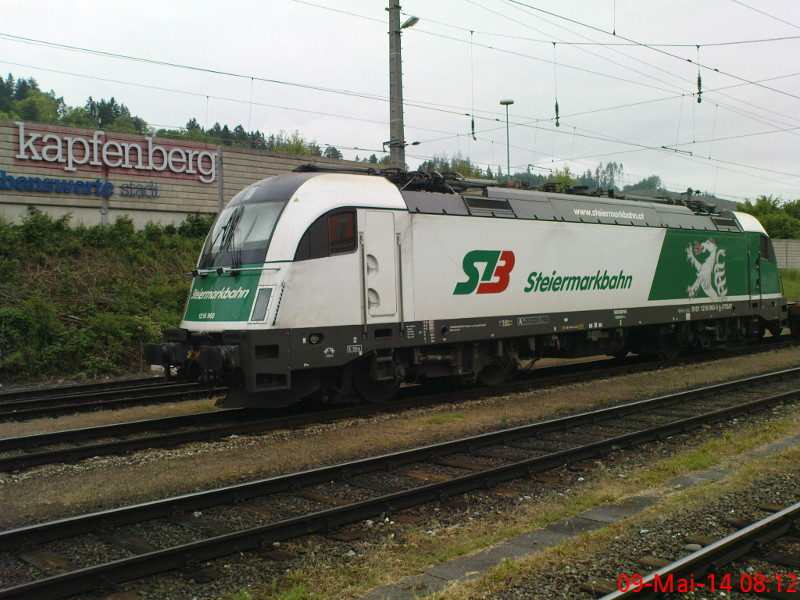
\includegraphics[keepaspectratio,width=0.95\textwidth]{images/engine}
  \caption[Logo at the train engine.]{Note the logo attached to the train engine spotted in Kapfenberg main station.}
  \label{fig:engine}
\end{figure}

Code listings require the \textit{listings} package which, in turn, requires some settings\footnote{\ldots because the defaults do not fit all purposes}; see command \verb+\lstset{}+ in preamble of this template. Additionally the package \textit{courier} should be used because the defaults do not provide for proper syntax highlighting.

\lstset{
caption={Listing subtitles could and should contain whole sentences describing the important aspect of the listing.}, 
basicstyle=\small\ttfamily, label=lst:main, language=C,frame=single}
%	basewidth={0.55em}, fontadjust}	% adjust these for more appealing appearance
\begin{lstlisting}
void main(int argc, char *argv[])
{
  printf("Hello world!");
}
\end{lstlisting}

In order to see what's possible -- here are two fancy tables, see Table~\ref{tab:olive} and Table~\ref{tab:grey} which show \ldots.

\begin{center}
  \begin{table}[tbp]
    \begin{tabular}{|l|l|l|l|}\hline
      \rowcolor{olivegreen30}
      \textcolor{white}{\textbf{Version}}
      	 &\textcolor{white}{\textbf{Description}}	
      	   &	\textcolor{white}{\textbf{Author(s)}}	
      	     &\textcolor{white}{\textbf{Date}}\\
      \hline
      1.0	
        & Initial				
          & Ohrt					
            & July 15, 2014\\
      \hline
      1.1	
        & Filled section ``Open Issues''	
          & Ohrt					
            & July 16, 2014\\
      \hline
      1.2	
        & Added section ``Restrictions''	
          & Ohrt					
            & September 15, 2014\\
      \hline
    \end{tabular}
    \caption{Olive green heading used for this fancy table.}
    \label{tab:olive}
  \end{table}
\end{center} 
  
View also the preamble of this file for explanations.
  
\begin{center} 
  \begin{table}[tbp]
    \begin{tabular}{ l | l }
      \rowcolor{gray20}\textbf{Error}	
        & \textbf{Solution} \\
      \rowcolor{gray5}Java.lang.OutOfMemoryError: PermGen space
        & -XX:MaxPermSize=1024M \\
      \rowcolor{gray5}\textit{(32-/64-bit issue)}
      	& \\
      \rowcolor{gray20}Error occurred during initialization of VM \textit{or}
      	& increase or remove -Xms value \\
      \rowcolor{gray20}Could not reserve enough space for object heap
      	& e.g.\ -Xms128m -Xmx512m \\
      \rowcolor{gray20}					
        & \small{(Eclipse default:}\\
      \rowcolor{gray20}					
        & \small{-Xms40m -Xmx512m)} \\
    \end{tabular}
    \caption{A more or less simple grey table. Better try to put tables and figures at \textit{top}[t] or \textit{bottom}[b] (optional use whole \textit{page}[p]) of a page. Avoid location specifier \textit{here}[h].}
    \label{tab:grey}
  \end{table}
\end{center}



Here is a reference to Listing~\ref{lst:main}. Note the line numbers. Referenced listings, tables and figures are written in uppercase first letter: \emph{L}isting X,  \emph{T}able Y and  \emph{F}igure Z.



\subsection{Prototype}

Find in Listing~\ref{lst:democlosure} an example of the JavaScript closure. Only parts of the original source code have been included. That allows to extract and display parts of working code!

\lstinputlisting[language=JavaScript,
 float=tbp,
 label=lst:democlosure, 
 firstline=10, 
 lastline=88, 
 caption={Demo implementation of a JavaScript \emph{Closure}.}
]{src/closure.js}

Mathematical expressions are rendered beautifully by \LaTeX. Now enjoy the first Maxwell equation 
\begin{math} 
  \text{rot} \vec{H} = \vec{J} + \frac{\partial \vec{D}}{\partial t} 
\end{math}.

Selected resources about scientific working: 

\begin{itemize}
  \item \emph{\citetitle{Zobel:2004}}: \ldots elements of good writing - clarity, simplicity, accuracy, and organization \ldots by \cite{Zobel:2004}.
  
  \item \emph{\citetitle{Yin:2013}}: \ldots offers comprehensive coverage of the design and use of the case study method as a valid research tool \ldots by \cite{Yin:2013}.

  \item \emph{\citetitle{Strunk:2000}}: \ldots first edition about 1935; includes a list of valuable recommendations: be clear, do not overwrite \ldots by \cite{Strunk:2000}.

  \item \emph{\citetitle{Field:2003}}: \ldots Planning an Experiment,	
Experimental Designs, Descriptive Statistics, Inferential Statistics \ldots Answering the Question 'So What?' \ldots by \cite{Field:2003}.

  \item \emph{\citetitle{Booth:2008}}: \ldots What Is Research? Creating a Relationship with Your Reader: Your Role, Finding a Good Research Problem \ldots by \cite{Booth:2008}.

  \item \emph{\citetitle{Alley:1998}}: 
  \ldots 
  your writing is the principle way in which people learn about your work.
  When you communicate well, you receive credit for your 
  \ldots 
  by \cite{Alley:1998}.

  \item \emph{\citetitle{Eco:2010}}: \ldots Warum muss man eine wissenschaftliche Abschlussarbeit schreiben und was ist sie? \ldots by \cite{Eco:2010}.

  \item \emph{\citetitle{Wisconsin:2004}}: \ldots you will find many instructional materials we've developed for our Writing Center teaching: Planning and Writing Research Papers, Creating an Argument,  \ldots by \cite{Wisconsin:2004}.


\end{itemize}

Finally, before starting to write you might take a look at some of these references.

\vfill

Final note: at the end of each chapter you might sum up the contents of the chapter in a sentence or two. Then you might tell the reader what will be presented in the upcoming section (to make her/him curious).


% next chapter: start at right side, if two-sided; else just flush page
\chapterend
     % remove this
  
  
  % add chapters as required. For example 
  
  %%%%%%%%%%%%%%%%%%%%%%%%%%%%%%%%%%%%%%%%%%%%%%%%%%%%%%%%%%%%%%%%%%%%%%%%%%%%%
\chapter{Introduction}\label{chap:intro}
%%%%%%%%%%%%%%%%%%%%%%%%%%%%%%%%%%%%%%%%%%%%%%%%%%%%%%%%%%%%%%%%%%%%%%%%%%%%%
\chapterstart

% Overall problem
% key questions to answer
% your approach, the method
% one/two hypotheses (idea of solution)

Your text here (what is the problem? what does not work well at the moment? what do people need?) \ldots

%%%%%%%%%%%%%%%%%%%%%%%%%%%%%%%%%%%%%%%%%%%%%%%%%%%%%%%%%%%%%%%%%%%%%%%%%%%%%
\section{Problem Statement}\label{sec:problem}
%%%%%%%%%%%%%%%%%%%%%%%%%%%%%%%%%%%%%%%%%%%%%%%%%%%%%%%%%%%%%%%%%%%%%%%%%%%%%

Your text here (what is the overall problem? give examples. motivate, why does someone needs (better/faster/different) solution to the problem described?) \ldots

%%%%%%%%%%%%%%%%%%%%%%%%%%%%%%%%%%%%%%%%%%%%%%%%%%%%%%%%%%%%%%%%%%%%%%%%%%%%%
\section{Research Questions}\label{sec:rq}
%%%%%%%%%%%%%%%%%%%%%%%%%%%%%%%%%%%%%%%%%%%%%%%%%%%%%%%%%%%%%%%%%%%%%%%%%%%%%

Your text here (focus on two to four main research questions and detail on them) \ldots

%%%%%%%%%%%%%%%%%%%%%%%%%%%%%%%%%%%%%%%%%%%%%%%%%%%%%%%%%%%%%%%%%%%%%%%%%%%%%
\section{Hypthesis}\label{sec:hypothesis}
%%%%%%%%%%%%%%%%%%%%%%%%%%%%%%%%%%%%%%%%%%%%%%%%%%%%%%%%%%%%%%%%%%%%%%%%%%%%%


Your text here ( a hypothesis -- a rough idea -- of how you think a solution might look like. How to possibly solve a given problem ) \ldots


%%%%%%%%%%%%%%%%%%%%%%%%%%%%%%%%%%%%%%%%%%%%%%%%%%%%%%%%%%%%%%%%%%%%%%%%%%%%%
\section{Method}\label{sec:method} % Materials and Methods
%%%%%%%%%%%%%%%%%%%%%%%%%%%%%%%%%%%%%%%%%%%%%%%%%%%%%%%%%%%%%%%%%%%%%%%%%%%%%

Your text here (your structured, academic approach\footnote{Find an extensive explanation of how to write a \emph{Method} section at \url{http://www.mrcophth.com/publishorperish/methods.html}.} to find a solution) \ldots


\chapterend

   % framing the problem 
                                       % research questions
                                       % hyptothesis
                                       % method
  
  %%%%%%%%%%%%%%%%%%%%%%%%%%%%%%%%%%%%%%%%%%%%%%%%%%%%%%%%%%%%%%%%%%%%%%%%%%%%%
\chapter{Analyse des Entwicklungsprozesses}\label{chap:related}
%%%%%%%%%%%%%%%%%%%%%%%%%%%%%%%%%%%%%%%%%%%%%%%%%%%%%%%%%%%%%%%%%%%%%%%%%%%%%
\chapterstart

Der gesamte Entwicklungsprozess umfasst 3 Teilbereiche:

\begin{itemize}

    \item Innovation
    \item Entwicklung
    \item Produktwartung

\end{itemize}

Es wird der Teilbereich der Entwicklung analysiert. Dieser Teilbereich umfasst folgende Aufgabengebiete:

\begin{itemize}

    \item Detailierte Spezifizierung der Anforderungen
    \item Systemdesign
    \item Umsetzung
    \item Testung des entwickelten Produkts
    \item Dokumentation und Schulung

\end{itemize}

Aus dem Bereich Innovation werden Anforderungen definiert die in der Produktentwicklung umgesetzt werden. Dabei sind qualitative, terminliche und budgetäre Rahmenbedingungen zu berücksichtigen. Entstandene Produkte müssen sich in die bestehende Systemlandschaft integrieren.

\section{Anforderungsdefinition}

Die Anforderungsdefinition ist ein erster Schritt, um aus einer ersten Idee, einem Kundenwunsch oder der Forderung nach einer neuen Technologie eine Entwicklung anzustoßen. 

\begin{figure}[h]
  \centering
  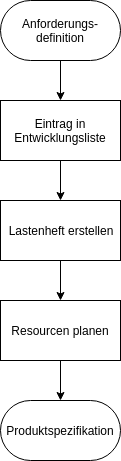
\includegraphics[keepaspectratio,height=0.8\textwidth]{images/3_2_1_1_Anforderungsdefinition_redraw.png}
  \caption[Anforderungsdefinition bis Produktspezifikation]{Die nötigen Tätigkeiten von der Anforderung bish zur Produktspezifikation.}
  \label{fig:Anforderungsdefinition}
\end{figure}

Es findet in diesem Schritt eine erste Bewertung des entsprechenden Entwicklungsvorschlags statt. Diese wird priorisiert und in die Entwicklungsliste eingetragen. Der Vorschlag wird danach in Form eines Lastenheftes dokumentiert und Ressourcen werden verplant. Hier kann es zu Verschiebungen von bereits priorisierten Entwicklungsprojekten kommen.

\section{Produktspezifikation}

Der \ac{TPL} leitet ein oder mehrere Workshops in denen die Anforderungen aus dem Lastenheft des \ac{PD} in Soft- und Hardware-Anforderungen ins Pflichtenheft umgesetzt werden. Dies geschieht mit der Unterstützung vom \ac{BDE} und \ac{BPI}. Die Gliederung der Anforderungen und die Zuordnung zu Soft bzw. Hardware-Subsystemen kann durch eine Use-Case-Analyse erfolgen.

Bei der Erstellung des Pflichtenhefts sollen möglichst Synergien der Soft- und Hardwarekomponenten genützt und die Möglichkeiten neuer Informationstechnologien ausgeschöpft werden. 

\begin{figure}[h]
    \centering
    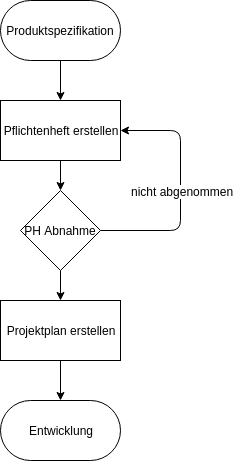
\includegraphics[keepaspectratio,height=0.8\textwidth]{images/3_2_1_2_Produktspezifiktation_redraw.png}
    \caption[Produktspezifikation bis Systemdesign]{Die nötigen Tätigkeiten von der Produktspezifikation bis zum Systemdesign.}
    \label{fig:Produktspezifiktation}
  \end{figure}

Sobald das Pflichtenheft erstellt wurde, wird ein Projektplan erstellt, um folgende Punkte zu definieren:

\begin{itemize}

    \item Abschätzung des Gesamtumfanges, -aufwandes und der Gesamtkosten
    \item Meilensteine 
    \item Iterationen und deren Ziele in den Phasen
    \item Zeitplan und Budget
    \item Zur Verfügung stehende Kapazitäten 
    \item Notwendige Aktivitäten für den korrekten Abschluss

\end{itemize}

Die Projektplanung erfolgt wiederum im Rahmen von ein oder mehreren Workshops. In diesen schätzt der \ac{TPL} mit Unterstützung durch die \ac{BDE}, \ac{BPI} und \ac{PD} den Aufwand, um das Projekt umsetzen zu können, und entwickelt einen Terminplan, der die Rahmenbedingungen des Projekts erfüllt.

Weiters werden die Meilensteine der Projektphasen festgelegt, an denen der Projektfortschritt beurteilt und die Aufwände und Kosten geprüft werden. Auf der Basis der Aufwandsschätzung und des Terminplans werden die benötigten Ressourcen definiert, um das Projekt umzusetzen. Der \ac{TPL} legt fest, welche Rollen und wie viele Ressourcen in welcher Projektphase benötigt werden.

Schließlich erstellt der \ac{TPL} einen Plan für die ordentliche Übergabe des Projekts und definiert die damit verbundenen Aktivitäten. Damit kann in die Entwicklungsphase übergegangen werden.

\section{Entwicklungs-Start}

Der Entwicklung-Start Prozess stellt sicher, dass in der nächsten Phase, der Entwicklungs-Umsetzung, alle notwendigen Informationen vorliegen und die Infrastruktur bereitsteht. 
Folgende Aspekte werden berücksichtigt:

\begin{itemize}
    \item Qualitätsüberprüfung der Anforderungen
    \item Bestimmung der Systemgrenzen
    \item Validierung der Aufwandsschätzung
    \item Abarbeitungsplan (Releaseplan)
    \item Ziele der Testung
    \item Überprüfung der Infrastruktur
\end{itemize} 

\subsection{Anforderungsreview}

Anforderungen wurden durch die \ac{PD} definiert. Vor der Entwicklungs-Umsetzung werden diese zu einem Termin von \ac{EPL}, Software Architekten und gegebenenfalls einzelnen Personen des Entwicklungsteams reviewed. 3 Aspekte sind zu klären:

\paragraph{Verständlichkeit:} 
Die Anforderungen müssen soweit klar, verständlich und widerspruchsfrei sein.

\paragraph{Umsetzbarkeit:} 
Die Anforderungen sind auf ihre technische Umsetzbarkeit hin zu überprüfen.

\paragraph{Vereinfachung:} 
Es ist zu klären, ob eine Änderung der Anforderungsbeschreibung die technische Umsetzung vereinfachen würde.

\subsection{Systemdesign erstellen}

Es werden die Systemgrenzen zu anderen Produkten des Unternehmens und externen zugekauften Produkten definiert. Daraus ergeben sich Schnittstellen zu den besagten Produkten. Diese Phase wird vorrangig von \ac{EPL}s oder Enterprise-Architekten vollzogen, kann jedoch auch von den Software-Architekten umgesetzt werden.

\subsection{Entwicklungs-Aufwände bestimmen}

Die Anforderungen sind bezüglich der Entwicklungs-Aufwände zu bewerten. Gemeinsam mit den geplanten Aufwänden für Koordination, Dokumentation, Tests, etc. sind die gesamten Entwicklungs-Aufwände grob zu planen.

\subsection{Release Planung}

Die geplanten Releases (Gruppierung von Anforderungen) sind mit Start-Datum und Ende-Datum zu definieren.
Die Zuteilung der Anforderungen zu Releases erfolgt gemeinsam mit dem Produktmanagement und der Software Entwicklung. Hier ist zu beachten, dass Releases in sinnvoller technischer Reihenfolge abgewickelt werden sollten. Weiters müssen die zur Verfügung stehenden Ressourcen bedacht werden.

\subsection{Entwicklungs-Infrastruktur erstellen}

In Abhängigkeit vom Systemdesign und dem gewählten Inventar an Umsetzungsmechanismen erstellt der \ac{EPL} bzw. der Architekt einen Plan für die Entwicklungsumgebung(en) und Testumgebung, in denen die Umsetzung erfolgt. Darin enthalten ist die Auswahl der Hardware- und Software-Komponenten sowie die nötige Infrastruktur (Build-Umgebung, Datenbank, Versionierung, Entwicklungsumgebung, etwaige andere Tools).

\section{Entwicklungs-Umsetzung}

Für die relevanten Anforderungen werden Design-Entscheidungen getroffen, Testfälle definiert, auf Basis des Designs implementiert, Testfälle durchgeführt und das Release ausgeliefert.

Dies wird in einem iterativem Verfahren abgehandelt, angelehnt an das Scrum Konzept werden Sprints definiert, um die Umsetzung voranzutreiben.

\subsection{Sprint}

Die Arbeit erfolgt in Iterationen von bis zu einem Monat. Jeder abgeschlossene Sprint soll einen konkreten Wert für den Kunden oder Benutzer erstellt haben. Die Länge des Sprints sollte konsistent bleiben. \parencite[vgl.][S. 62]{Rubin:2012}

Die Sprintplannung erfolgt zu einem Termin, an dem über den Inhalt und die Umsetzungsdetails beraten wird. \parencite[vgl.][S. 339]{Rubin:2012} Zu diesem Zeitpunkt werden auch Testfälle spezifiziert.

\subsection{Release-Übergabe und Abnahme}

Die fertige Software wird an das Produktmanagement bzw. den Produktverantwortlichen übergeben. Der Umfang der Software ist in den Release-Notes dokumentiert. Diese beinhalten zumindest die umgesetzten Anforderungen, die behobenen Fehlerfälle, neu eingeführte Parameter und ggf. bekannte Probleme. 

Das Produktmanagement bzw. den Produktverantwortlichen prüft gemeinsam mit der Entwicklung die übergebene Release anhand der Anforderungen und prüft die übergebene Dokumentation. Werden die Anforderungen erfüllt, ist die Entwicklung abgenommen und somit freigegeben; falls nicht alle Anforderungen erfüllt werden, muss die Entwicklung die fehlenden oder nicht fehlerfreien Teile nachliefern.

\subsection{Produkt Schulung}

Bei Bedarf (initiiert von den Produktmanagern bzw. dem Produktverantwortlichen) werden die neuen Features vorgestellt und die Anwender (Projekt-Entwickler, bzw. -Abwickler) geschult.

\subsection{Produkt Review}
Nach dem ersten Einsatz der Release kann eine Produkt Review eingeleitet werden. Ziel ist es, für zukünftige Projekte, Verbesserungspotential zu finden.

\section{System-Test}

Ein Mitarbeiter des Bereiches \ac{BDE} bzw. \ac{BPI} testet die aus der Umsetzung entstandene Software zusammen mit allen notwendigen Fremdgewerken entsprechend des Testplans und füllt die Testprotokolle mit den gewonnen Ergebnissen aus. Entscheidend dabei ist, dass im Test entstandene Fehler auf ihre Reproduzierbarkeit überprüft werden. Eventuell muss der Testplan entsprechend angepasst werden, damit der Entwickler in der Lage ist, den Fehler zu reproduzieren und zu beseitigen.

\begin{figure}[h]
    \centering
    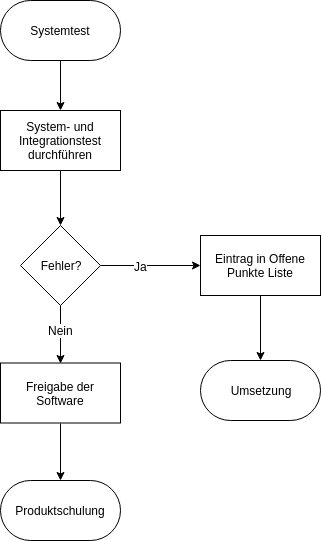
\includegraphics[keepaspectratio,height=0.9\textwidth]{images/3_2_1_5_Systemtest_redraw.png}
    \caption[Systemtest]{Der Ablauf der Systemtests.}
    \label{fig:Produktspezifiktation}
\end{figure}

\section{Produkt-Schulung}

Der \ac{TPL} organisiert für jede Zielgruppe (\ac{BPI}, \ac{PD}) ein oder mehrere Workshops, in denen von der \ac{BDE} bzw. \ac{BPI} die Anwendung der Software mithilfe der erstellten Unterlagen geschult wird. Die Teilnehmer dieser Workshops sind dann in der Lage, die notwendigen Tätigkeiten für das Produkt-Rollout durchzuführen und können die End-Anwender schulen.



\chapterend        % research related (to your!) work 
  %%%%%%%%%%%%%%%%%%%%%%%%%%%%%%%%%%%%%%%%%%%%%%%%%%%%%%%%%%%%%%%%%%%%%%%%%%%%%
\chapter{Konzept}\label{chap:concept}
%%%%%%%%%%%%%%%%%%%%%%%%%%%%%%%%%%%%%%%%%%%%%%%%%%%%%%%%%%%%%%%%%%%%%%%%%%%%%
\chapterstart

Der aktuell implementierte Prozess ist in den Phasen Entwicklung und Systemtest bereits agil konzipiert. 
Der Ablauf der Anforderungsdefinition, Produktspezifikation und dem Entwicklungs-Start sind einem klassischen Wasserfallmodell nachempfunden. Vor allem die Anforderungsdefinition ist die große Hürde, da hier bereits die Anforderungen recht detailreich vertraglich beschlossen werden.

Dies steht im Gegensatz zum agilen Manifest, welches in seinen 4 Punkten das allgemeine Gesamtverhalten beschreibt. 

\textbf{Individuals and interactions} over processes and tools \\
\textbf{Working software} over comprehensive documentation \\
\textbf{Customer collaboration} over contract negotiation \\
\textbf{Responding to change} over following a plan \\ \parencite{Beck:2001}

Um den gesamten Prozess agiler gestalten zu können, muss das agile Konzept über die Entwicklungs-Umsetzung hinaus adaptiert werden. 

\section{Agile Produktspezifikation}

Laut Rubin soll man nicht davon ausgehen, dass man die Pläne zu Beginn bereits richtig definieren kann. Es werden keine Optionen offen gelassen. \parencite[vgl.][S. 248, 249]{Rubin:2012} Die Erstellung des Pflichtenheftes und des Projektplans fordern jedoch genau das. Meilensteine, Zeitpläne und notwendige Aktivitäten für den korrekten Abschluss sind zu diesem Zeitpunkt bereits definiert.

Um dem entgegenzuwirken, sollte die Produktspezifikation Teil des Scrum Prozesses werden. In jedem Sprint trifft sich der Produktverantwortliche mit dem Entwicklungsteam um über die nächsten Anforderungen im Sprint einzulasten. Ein Vorteil dieser Methode ist, da der Produktverantwortliche zu Beginn noch nicht im Klaren über die genau Anforderung ist, dass das sich entwickelnde System mehr Klarheit über die Anforderungen schafft. Außerdem hat das Entwicklungsteam durch den direkten Zugriff zum Produktverantwortlichen die Möglichkeit, die Anforderung besser verstehen zu können. \parencite[vgl.][S. 27]{Ramadan:2016}

Im Fallbeispiel bedeute dies konkret, dass \ac{PD} Teil des Scrum-Teams wird. Es würd kein Pflichtenheft vorab mehr geschrieben werden, sondern das Pflichtenheft würde in jeder Iteration erweitert und detailreicher spezifiziert werden.

Die große Hürde dieser Umstellung ist jedoch die vertragliche Regelung, die bereits in der Anforderungsdefinition beginnt. Aus der Analyse geht hervor, dass mit Abschluss des Pflichtenheftes der Vertrag zustande gekommen ist. Dies ist der Zeitpunkt an dem terminliche Fixpunkte definiert werden. Ebenso die Aufwandsschätzung ist hier abgeschlossen. Um diese Hürde bewältigen zu können, benötigt es einer anderen Form der vertraglichen Regelung. Einen agilen Vertrag.

\section{Agiler Vertrag}

An agile fixed-price contract defines a contractual framework within which time and costs are agreed upon, as well as a structured approach to steer the scope within boundaries and by processes in a defined and controlled manner. Thus, the contractual structure of an agile fixed-price contract reacts to two uncertainties. On the one hand, you never know exactly what details will be needed at the start of a project. On the other hand, you do not always need everything that had originally been considered to be important. \parencite[S. 47]{Opelt:2013}

Für die Umsetzung eines agilen Vertrages, bedarf es eines Änderungswillen im gesamten Unternehmen und den Willen des Kunden agile Methodiken einzusetzen. Wenn dieser vorhanden ist, bedarf es keiner Pflichtenheft Erstellung mehr. Die Anforderungsdefinition kann auf ein Minimum reduziert werden da zu Beginn Anforderungen nur auf einem hohen Abstraktionsniveau definiert werden.

\chapterend        % concept/design of solution
  %%%%%%%%%%%%%%%%%%%%%%%%%%%%%%%%%%%%%%%%%%%%%%%%%%%%%%%%%%%%%%%%%%%%%%%%%%%%%
\chapter{Implementation}\label{chap:implementation}
%%%%%%%%%%%%%%%%%%%%%%%%%%%%%%%%%%%%%%%%%%%%%%%%%%%%%%%%%%%%%%%%%%%%%%%%%%%%%
\chapterstart

Your text here (describe what is relevant and special about your working prototype, state how the single features help to solve the given problem) \ldots




\chapterend % implementation, prototype
  %%%%%%%%%%%%%%%%%%%%%%%%%%%%%%%%%%%%%%%%%%%%%%%%%%%%%%%%%%%%%%%%%%%%%%%%%%%%%
\chapter{Evaluation}\label{chap:evaluation}
%%%%%%%%%%%%%%%%%%%%%%%%%%%%%%%%%%%%%%%%%%%%%%%%%%%%%%%%%%%%%%%%%%%%%%%%%%%%%
\chapterstart

Your text here (describe, how you could prove, that your implementation really solved the stated problem. I.e. accept or reject your hypotheses) \ldots

\chapterend
     % evaluation of prototype
  %%%%%%%%%%%%%%%%%%%%%%%%%%%%%%%%%%%%%%%%%%%%%%%%%%%%%%%%%%%%%%%%%%%%%%%%%%%%%
\chapter{Fazit}\label{chap:conclusion}
%%%%%%%%%%%%%%%%%%%%%%%%%%%%%%%%%%%%%%%%%%%%%%%%%%%%%%%%%%%%%%%%%%%%%%%%%%%%%
\chapterstart

Das Fallbeispiel implementiert agile Methodiken in einem kleinen Bereich im gesamten Entwicklungsprozess. Nur Prozesse, die direkt mit dem Entwicklungsteam in Kontakt kommen, sind agil konzipiert.

Eine Ausweitung agiler Methodiken wäre durchaus möglich. Im ersten, einfachen, Schritt kann die Produktspezifikation in den Scrum-Prozess ohne große Probleme eingeführt werden. Bestehende Abläufe müssten nur gering geändert werden. Der große Unterschied bestünde aus der Nähe des \ac{PD} zum Entwicklungsteam. Die Änderung könnte ohne große Hürden im Unternehmen umgesetzt werden. Somit wäre es sinnvoll, dies in einer Probephase zu erproben.

Die weitaus schwierigere Aufgabe ist es, die Idee eines agilen Vertrages im Unternehmens durchzusetzen. Juristische Expertise ist hier gefragt um rechtliche Sicherheit weiterhin gewährleisten zu können. Eine Einführung könnte aber große Effizienz- und Zufriedenheitssteigerungen mit sich bringen.  

\chapterend
     % summary, your conclusions/outlook

  \appendix
  %%%%%%%%%%%%%%%%%%%%%%%%%%%%%%%%%%%%%%%%%%%%%%%%%%%%%%%%%%%%%%%%%%%%%%%%%%%%%
\chapter*{Acronyms}
\label{chap:acronyms}
%%%%%%%%%%%%%%%%%%%%%%%%%%%%%%%%%%%%%%%%%%%%%%%%%%%%%%%%%%%%%%%%%%%%%%%%%%%%%
% Which one will be the longest ...?
% ABCDE --> \begin{acronym}[ABCDE]
\footnotesize
\begin{acronym}[ABCDE]
  \acro{ABI}{application binary interface}
  \acro{ACL}{access control list}
  \acro{GUI}{graphical user interface}
  \acro{KISS}{keep it small and simple}
  \acro{MITM}{man-in-the-middle}
  \acro{OS}{operating system}
  \acro{UART}{universal asynchronous receiver/transmitter}
  \acro{UID}{unique identifier}
\end{acronym}
\normalsize
       % optional

\printbibliography
% Add bibliography to table of contents as "References", at chapter level
% Keep this _after_ bibliography, only then the link in the TOC is correct!
\addcontentsline{toc}{chapter}{References}

\end{document}


%**********************************************************************
%**********************************************************************
